\documentclass{if-beamer}

% --------------------------------------------------- %
%                  Presentation info	              %
% --------------------------------------------------- %
\title[Projeto -- Etapa 2]{Arquitetura HIL para teste de sistemas embarcados como \textit{vehicle interface} de veículos autônomos baseados no Autoware}
\subtitle{Projeto -- Etapa 2}

\author[G. Toffanetto, J. L. Barraza]{\texorpdfstring
	{Gabriel Toffanetto França da Rocha 
		\\ \vspace{1mm} 
		\small{\href{mailto:g289320@dac.unicamp.br}{g289320@dac.unicamp.br}}
	}
	{Gabriel Toffanetto França da Rocha} \\
	\normalsize \vspace{2mm}
	Juan Luis Barraza Ramirez \\
	\small \vspace{1mm} j272583@dac.unicamp.br
}

\institute[LMA/FEM/Unicamp]{\small{Professor Dr. Rodrigo Moreira Bacurau
  \\ \vspace{2mm}
  IM420X -- Projeto de Sistemas Embarcados de Tempo Real
  \\ \vspace{4mm}
  Faculdade de Engenharia Mecânica
  \\ \vspace{1mm}
  Universidade Estadual de Campinas}
}

\date{22 de outubro de 2024}

\logo{
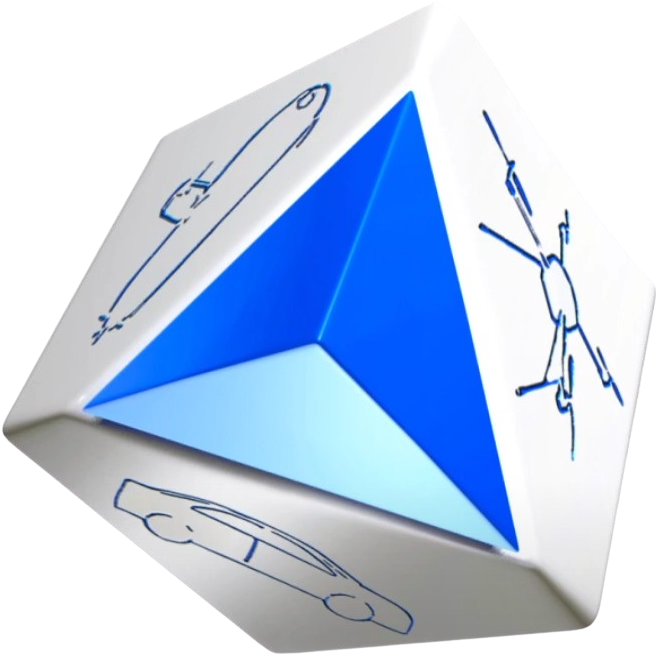
\includegraphics[width=1.2cm]{img/core/Logo_LMA_icon.png}
}


\subject{IM420X - Projeto final: Etapa 2} % metadata

\graphicspath{{img/}}

\setbeamertemplate{caption}[numbered]

\newcolumntype{b}{>{\columncolor{white}}c}


\hypersetup{pdfpagemode=FullScreen}


% --------------------------------------------------- %
%                    Title + Schedule                 %
% --------------------------------------------------- %

\begin{document}

\begin{frame}
  \titlepage
\end{frame}

\begin{frame}{Schedule}
  \tableofcontents
\end{frame}

% --------------------------------------------------- %
%                      Presentation                   %
% --------------------------------------------------- %

\section{Introdução}

\begin{frame}{Proposta}
	
	\begin{columns}
		
		\begin{column}{0.7\textwidth}
			
				\begin{figure}[H]
				\centering
				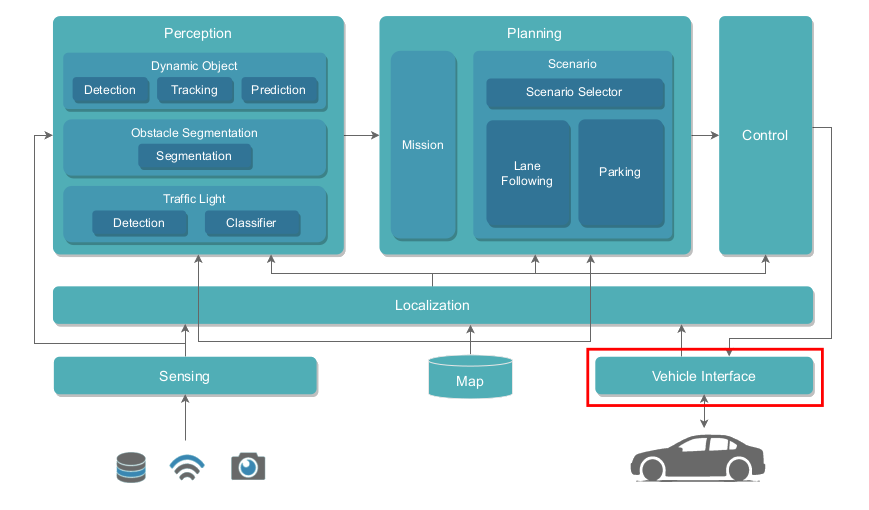
\includegraphics[width=\linewidth]{img/architecture.png}
				\caption{Escopo do projeto na arquitetura Autoware.}
				\label{fig:architecture}
			\end{figure}
			
		\end{column}
		
		\hspace{-0.5cm}
		
		\begin{column}{0.5\textwidth}
			
				\begin{figure}[H]
				\centering
				\includegraphics[width=\linewidth]{img/architecture_HIL}
				\caption{Arquitetura de teste do \textit{hardware}.}
				\label{fig:architecture_HIL}
			\end{figure}
			
		\end{column}
		
	\end{columns}
	
\end{frame}


\section{Tarefas}



\begin{frame}{Diagrama do sistema}
	
	% TODO: \usepackage{graphicx} required
	\begin{figure}
		\centering
		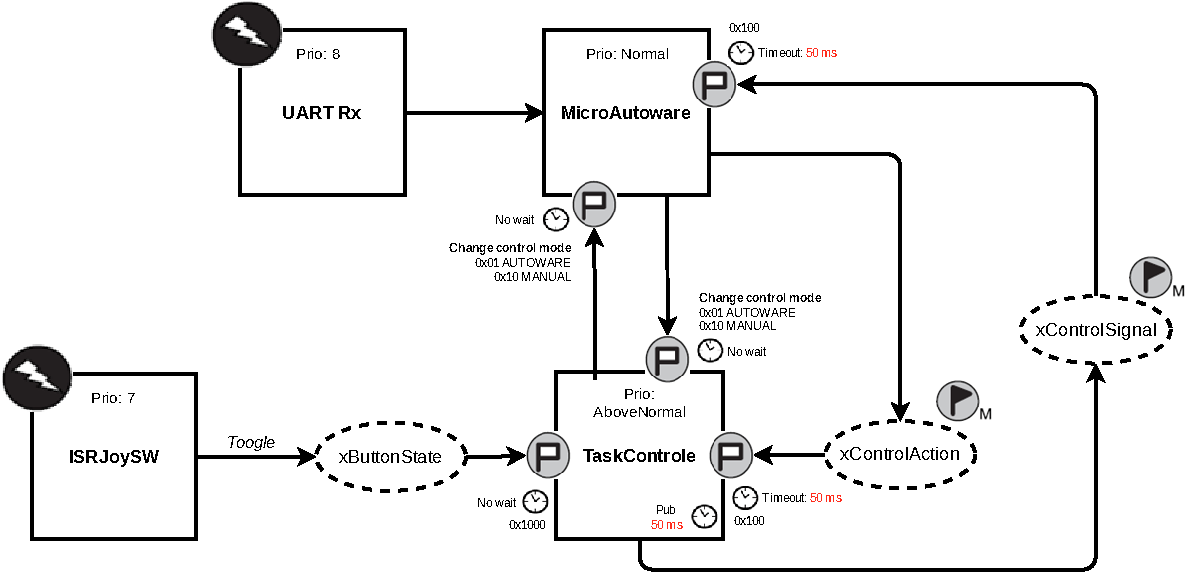
\includegraphics[width=0.75\linewidth]{img/system_diagram}
		\caption{Diagrama do sistema.}
		\label{fig:systemdiagram}
	\end{figure}
	
\end{frame}



\begin{frame}{Descrição das tarefas}
	
	
	
\end{frame}




\begin{frame}{Fluxograma das tarefas}
	
	
	
\end{frame}



\section{Sincronização e comunicação entre tarefas}

\begin{frame}{Troca do modo de controle -- Autoware}
	
	
	
\end{frame}

\begin{frame}{Troca do modo de controle -- Joystick}



\end{frame}

\begin{frame}{Envio da ação de controle de alto nível}



\end{frame}

\begin{frame}{Envio da ação de controle de baixo nível}



\end{frame}


\section{Cronograma}

\begin{frame}{Cronograma}
	
	
\begin{table}
	\centering
	\small{
		\begin{tabular}{|b|b|b|b|b|b|b|b|b|b|}
			\hline
			\textbf{Atividade/Semana} & 1 \cellcolor{lightgray} & \textbf{2} \cellcolor{lightgray} & 3 \cellcolor{lightgray} & \textbf{4} & 5 & 6 & \textbf{7} & 8 & \textbf{9} \\
			\hline
			Proposta do projeto  & \cellcolor{unifeiblue} &  &  &  &  &  &  &  &  \\
			\hline
			Projeto de \textit{hardware} e \textit{software}  &  & \cellcolor{unifeiblue} & \cellcolor{unifeiblue} &  &  &  &  &  &  \\
			\hline
			Integração do STM com o micro-ROS  &  & \cellcolor{unifeiblue} &  &  &  &  &  &  &  \\
			\hline
			Integração do micro-ROS com o Autoware  &  &  & \cellcolor{unifeiblue} & \cellcolor{unifeiblue} & \cellcolor{unifeiblue} &  &  &  &  \\
			\hline
			Implementação das tarefas do sistema embarcado  &  &  &  & \cellcolor{unifeiblue} & \cellcolor{unifeiblue} & \cellcolor{unifeiblue} & \cellcolor{unifeiblue} &  &  \\
			\hline
			Construção do ambiente de testes  &  &  &  &  & \cellcolor{unifeiblue} & \cellcolor{unifeiblue} & \cellcolor{unifeiblue} &  &  \\
			\hline
			Realização dos testes  &  &  &  &  &  &  & \cellcolor{unifeiblue} & \cellcolor{unifeiblue} & \cellcolor{unifeiblue} \\
			\hline
			Escrita do relatório  &   & \cellcolor{unifeiblue} & \cellcolor{unifeiblue} & \cellcolor{unifeiblue} & \cellcolor{unifeiblue} & \cellcolor{unifeiblue} & \cellcolor{unifeiblue} & \cellcolor{unifeiblue} & \cellcolor{unifeiblue} \\
			\hline
		\end{tabular}
	}
	\caption{Cronograma de atividades.}
	\label{tab:crono}
\end{table}
	
	\begin{itemize}
		\small
		\item \textbf{Semana 2:} Apresentação Etapa 1
		\item \textbf{Semana 4:} Apresentação Etapa 2
		\item \textbf{Semana 7:} Apresentação Etapa 3
		\item \textbf{Semana 9:} Apresentação Final
	\end{itemize}
	
\end{frame}


% -------------------------------------------------
%               Bibliografia.
%--------------------------------------------------
\section{Referências bibliográficas}
\begin{frame}{Referências bibliográficas}
   %\bibliographystyle{acm}
   \bibliography{bibliografia.bib}
\end{frame}



\begin{frame}{}
	
	\begin{block}{}
		
		\centering
		\Huge{Obrigado!}
		
		\LARGE
		
		\vspace{5mm}
		
		Dúvidas?
		
	\end{block}
	
	\vspace{4mm}
	
	\begin{figure}[H]
		\centering
		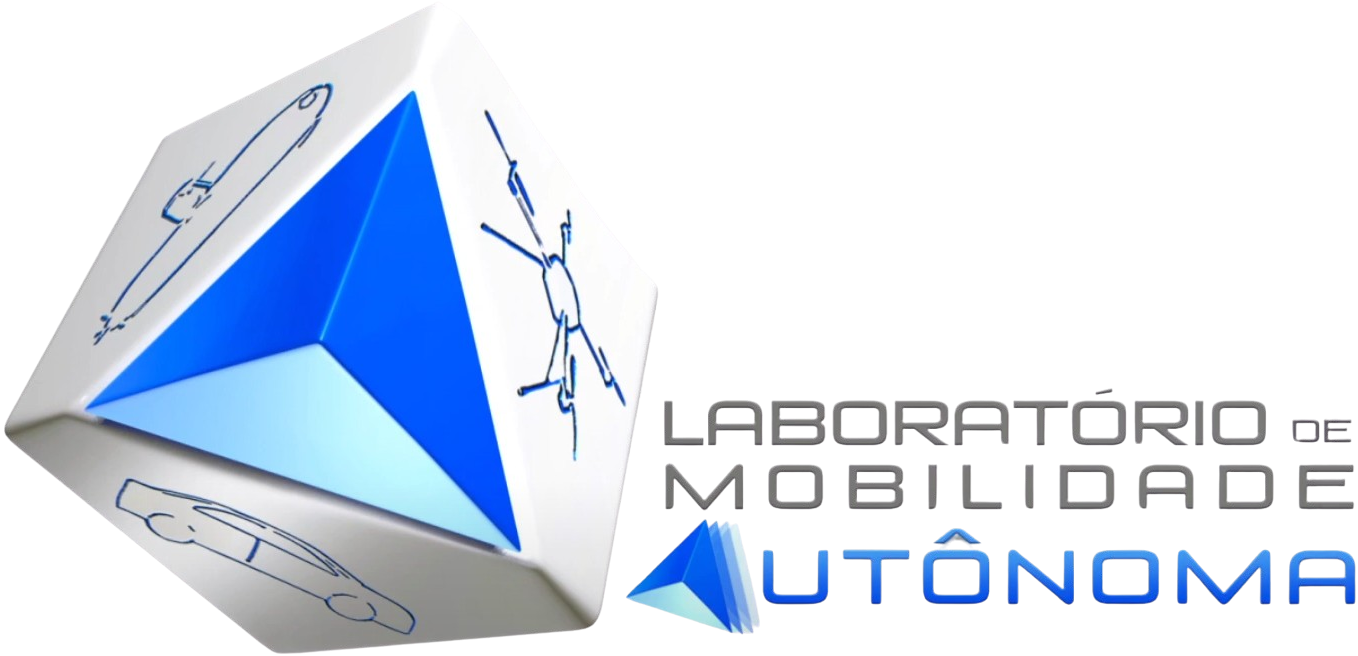
\includegraphics[width=0.5\linewidth]{img/core/Logo_LMA.png}
	\end{figure}
	
\end{frame}

\end{document}
